\documentclass[10pt,journal,compsoc,onecolumn, draftclsnofoot]{IEEEtran}

\usepackage{graphicx}
\usepackage{amssymb}
\usepackage{amsmath}
\usepackage{amsthm}
\usepackage{caption}

\usepackage{alltt}
\usepackage{float}
\usepackage{color}
\usepackage{url}

\usepackage{balance}
\usepackage[TABBOTCAP, tight]{subfigure}
\usepackage{enumitem}
\usepackage{pstricks, pst-node}

\usepackage{geometry}
\usepackage{pst-gantt}
\usepackage{tabu}

\usepackage{pdfpages}

\geometry{textheight=8.5in, textwidth=6in}

%random comment

\newcommand{\cred}[1]{{\color{red}#1}}
\newcommand{\cblue}[1]{{\color{blue}#1}}

\graphicspath{ {diagrams/} }

\usepackage{hyperref}
\usepackage{geometry}
\usepackage{array}
\usepackage{titling}

\def\name{Jake Jeffreys, McKenna Jones, Spike Madden, Sean Marty}
\title{
EmbarkVR: Outdoor Virtual Reality Experience \\
CS Senior Capstone \\
Final Report\\
\vspace{1mm}
}
\author{Jake Jeffreys, McKenna Jones, Spike Madden, Sean Marty}
\date{May 31, 2017}

%pull in the necessary preamble matter for pygments output

%% The following metadata will show up in the PDF properties
\hypersetup{
  colorlinks = true,
  linkcolor = black,
  urlcolor = black,
  pdfauthor = {\name},
  pdfkeywords = {``senior capstone''},
  pdftitle = {CS Capstone Report},
  pdfsubject = {CS Capstone Report},
  pdfpagemode = UseNone
}

\begin{document}
\begin{titlepage}
\maketitle
\vspace{1mm}
\begin{abstract}

\end{abstract}
\vspace{1cm}

\end{titlepage}
% \tableofcontents
% \let\tableofcontents\relax
\clearpage

\section{Original Requirements Document}
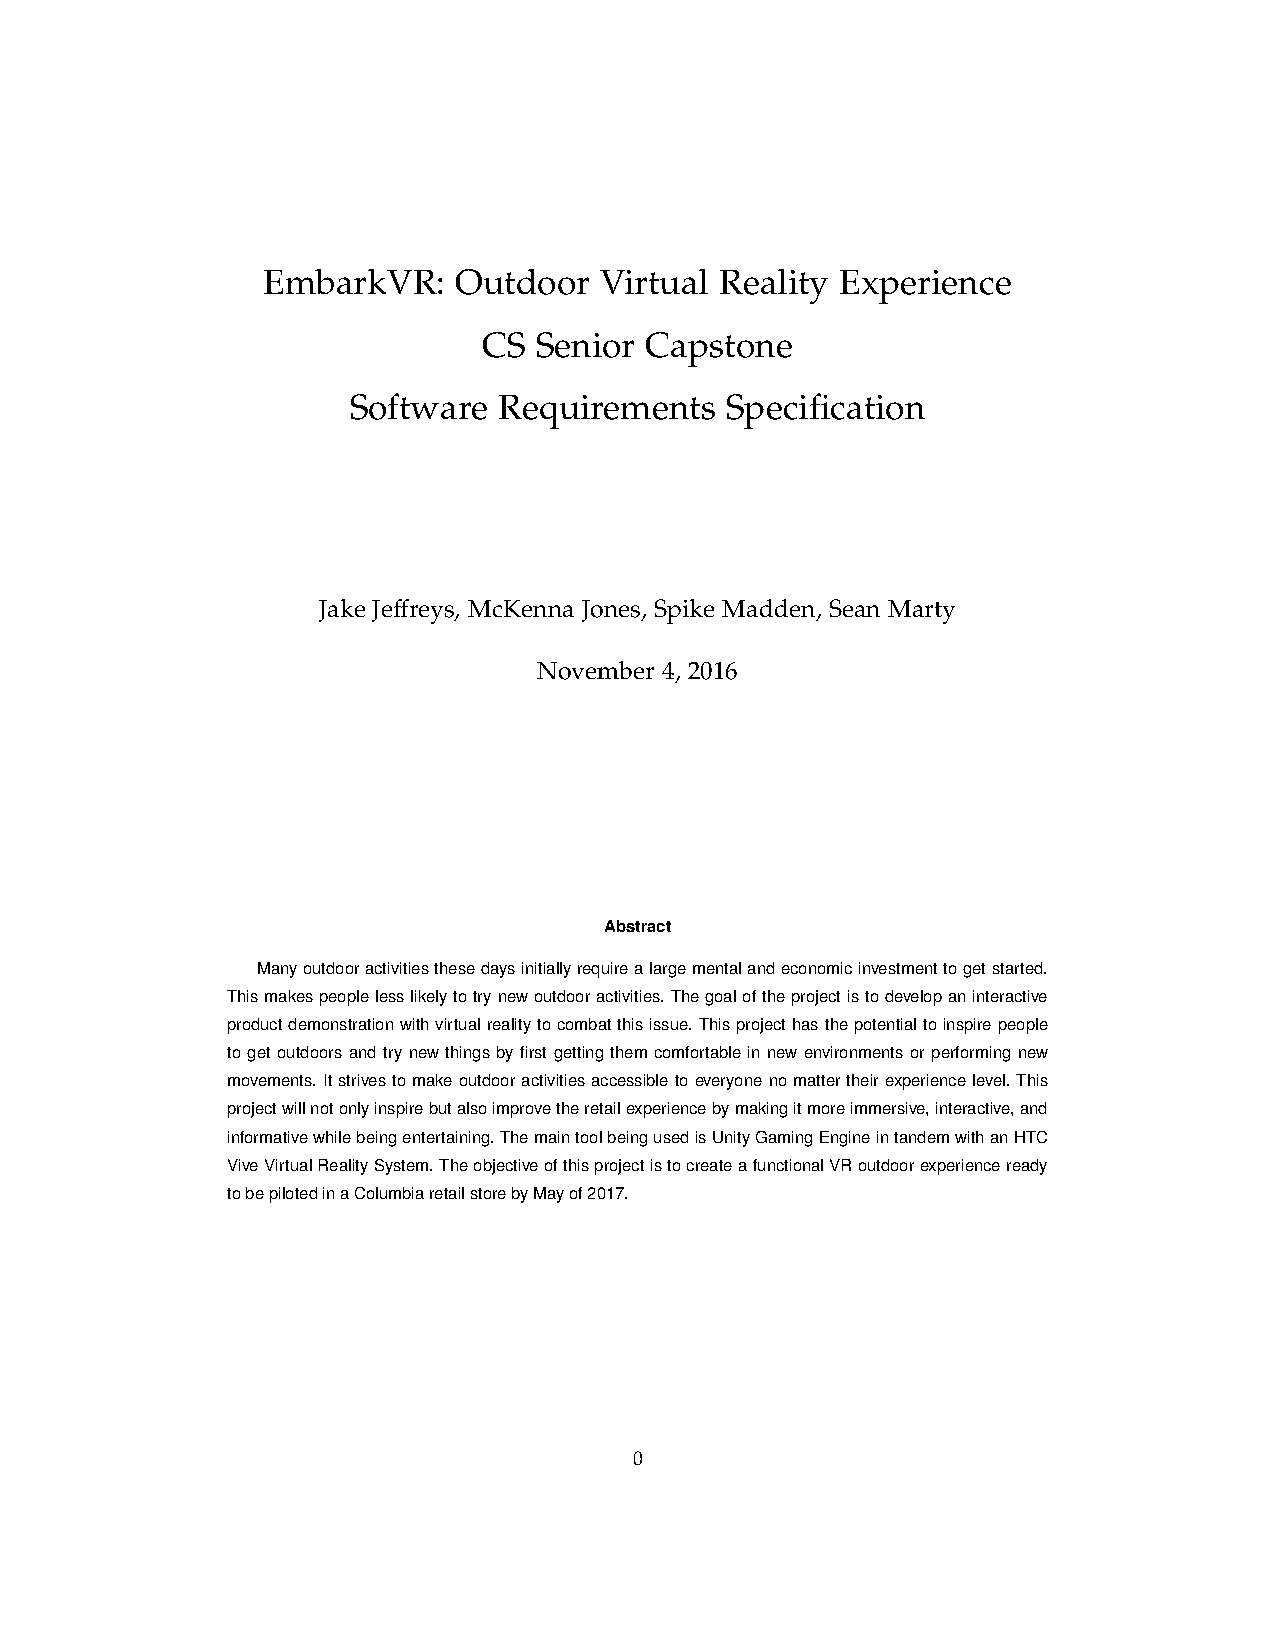
\includepdf[pages=-, frame, scale=0.9, pagecommand={}]{originalRequirementsDoc.pdf}
\section{How Have Requirements Changed?}

\section{Original Design Document}
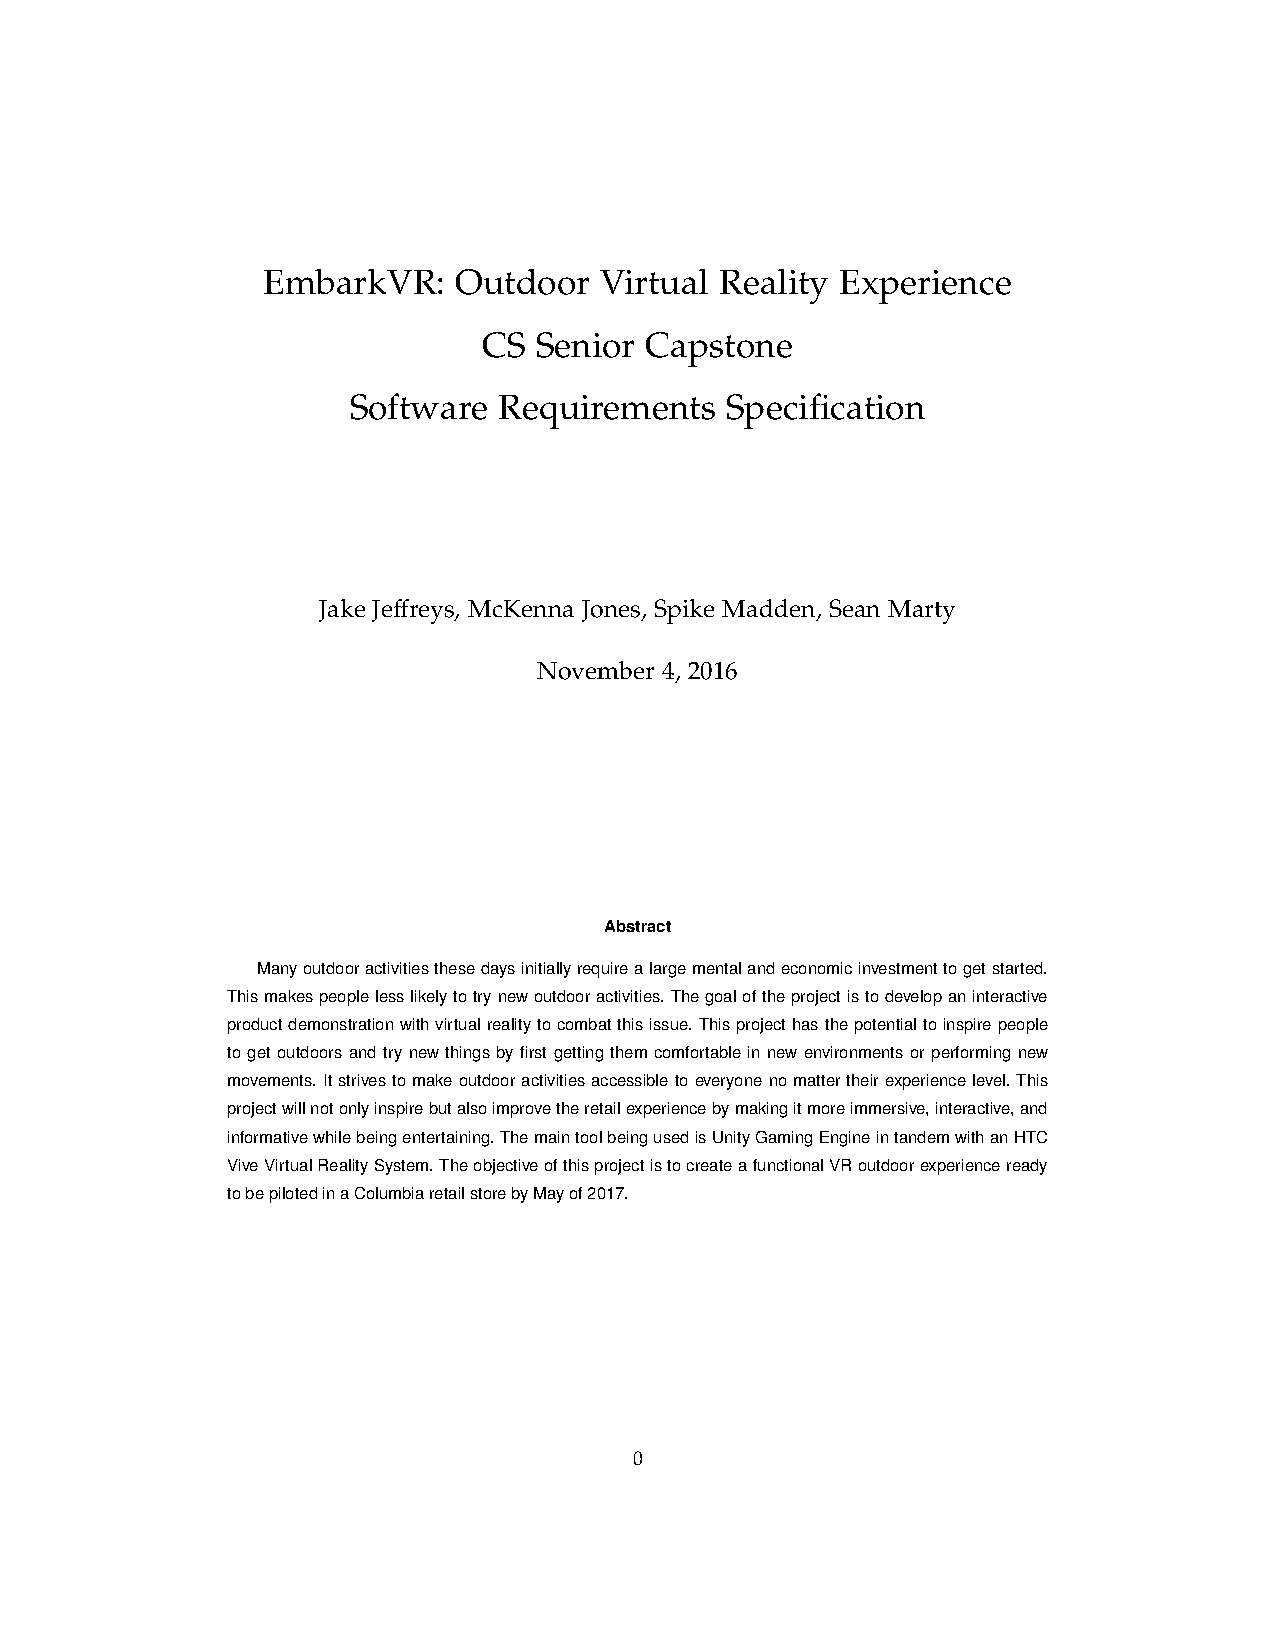
\includepdf[pages=-, frame, scale=0.9, pagecommand={}]{originalDesignDoc.pdf}

\section{Original Tech Review}
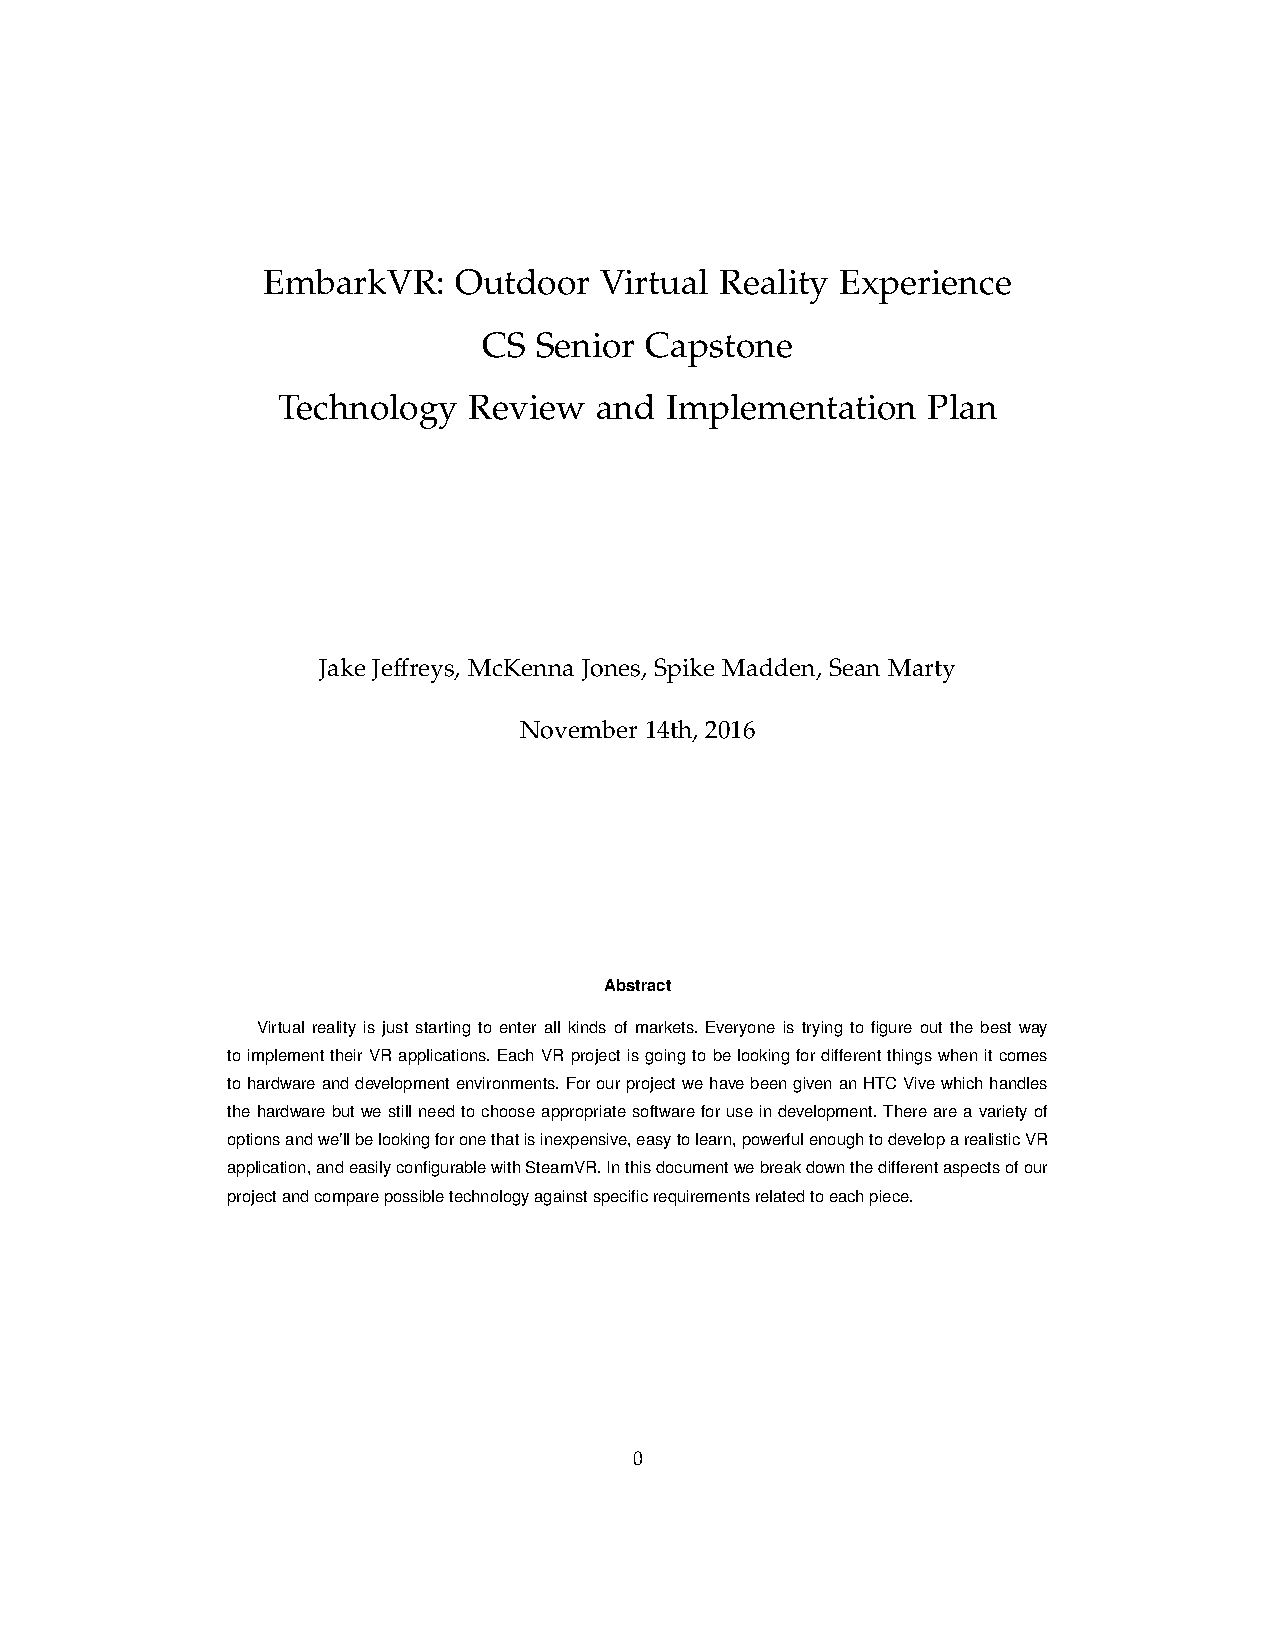
\includepdf[pages=-, frame, scale=0.9, pagecommand={}]{originalTechReview.pdf}

\section{Weekly Blog Posts}

\section{Final Expo Poster}

\section{Project Documentation}
\subsection{Technical Overview}
\subsection{How to Install}
\subsection{Running the Experience}
\subsection{Hardware Requirements}

\section{How We Learned}

\section{What We Learned}

% \bibliographystyle{IEEEtran}
% \bibliography{}
\end{document}
